\documentclass[12pt]{report}
\usepackage[spanish]{babel}
\usepackage[utf8]{inputenc}
\usepackage{amsmath}
\usepackage{amssymb}
\usepackage{amsthm}
\usepackage[mathscr]{euscript}
\usepackage{graphics}
\usepackage{wrapfig}
\usepackage{subfigure}
\usepackage{lipsum}
\usepackage{array}
\usepackage{multicol}
\usepackage{enumerate}
\usepackage[framemethod=TikZ]{mdframed}
\usepackage[a4paper, margin = 1.5cm]{geometry}
\usepackage{bbm}
\usepackage{float}

%En esta parte se hacen redefiniciones de algunos comandos para que resulte agradable el verlos%

\renewcommand{\theenumii}{\roman{enumii}}

\def\proof{\paragraph{Demostración:\\}}
\def\endproof{\hfill$\blacksquare$}

\def\sol{\paragraph{Solución:\\}}
\def\endsol{\hfill$\square$}

%En esta parte se definen los comandos a usar dentro del documento para enlistar%

\newtheoremstyle{largebreak}
  {}% use the default space above
  {}% use the default space below
  {\normalfont}% body font
  {}% indent (0pt)
  {\bfseries}% header font
  {}% punctuation
  {\newline}% break after header
  {}% header spec

\theoremstyle{largebreak}

\newmdtheoremenv[
    leftmargin=0em,
    rightmargin=0em,
    innertopmargin=-2pt,
    innerbottommargin=8pt,
    hidealllines = true,
    roundcorner = 5pt,
    backgroundcolor = gray!60!red!30
]{exa}{Ejemplo}[section]

\newmdtheoremenv[
    leftmargin=0em,
    rightmargin=0em,
    innertopmargin=-2pt,
    innerbottommargin=8pt,
    hidealllines = true,
    roundcorner = 5pt,
    backgroundcolor = gray!50!blue!30
]{obs}{Observación}[section]

\newmdtheoremenv[
    leftmargin=0em,
    rightmargin=0em,
    innertopmargin=-2pt,
    innerbottommargin=8pt,
    rightline = false,
    leftline = false
]{theor}{Teorema}[section]

\newmdtheoremenv[
    leftmargin=0em,
    rightmargin=0em,
    innertopmargin=-2pt,
    innerbottommargin=8pt,
    rightline = false,
    leftline = false
]{propo}{Proposición}[section]

\newmdtheoremenv[
    leftmargin=0em,
    rightmargin=0em,
    innertopmargin=-2pt,
    innerbottommargin=8pt,
    rightline = false,
    leftline = false
]{cor}{Corolario}[section]

\newmdtheoremenv[
    leftmargin=0em,
    rightmargin=0em,
    innertopmargin=-2pt,
    innerbottommargin=8pt,
    rightline = false,
    leftline = false
]{lema}{Lema}[section]

\newmdtheoremenv[
    leftmargin=0em,
    rightmargin=0em,
    innertopmargin=-2pt,
    innerbottommargin=8pt,
    roundcorner=5pt,
    backgroundcolor = gray!30,
    hidealllines = true
]{mydef}{Definición}[section]

\newmdtheoremenv[
    leftmargin=0em,
    rightmargin=0em,
    innertopmargin=-2pt,
    innerbottommargin=8pt,
    roundcorner=5pt
]{excer}{Ejercicio}[section]

%En esta parte se colocan comandos que definen la forma en la que se van a escribir ciertas funciones%

\newcommand\abs[1]{\ensuremath{\left|#1\right|}}
\newcommand\divides{\ensuremath{\bigm|}}
\newcommand\cf[3]{\ensuremath{#1:#2\rightarrow#3}}
\newcommand\natint[1]{\ensuremath{\left[\!\left[ #1\right]\!\right]}}
\newcommand{\afa}{\:
    \begin{tikzpicture}
        \draw [line width = 0.17 mm, black] (0,0) -- (-0.115,0.29);
        \draw [line width = 0.17 mm, black] (0,0) -- (0.115,0.29);
        \draw [line width = 0.17 mm, black] (-0.12,0) arc (190:-10:0.12cm);
    \end{tikzpicture}
    \:
}
%Este símvolo es para casi todo salvo una cantidad finita

%recuerda usar \clearpage para hacer un salto de página

\begin{document}
    \setlength{\parskip}{5pt} % Añade 5 puntos de espacio entre párrafos
    \setlength{\parindent}{12pt} % Pone la sangría como me gusta
    \title{Notas Taller Topología Algebraica}
    \author{Cristo Daniel Alvarado}
    \maketitle

    \tableofcontents %Con este comando se genera el índice general del libro%

    \setcounter{chapter}{1} %En esta parte lo que se hace es cambiar la enumeración del capítulo%
    
    \chapter{Grupos Libres y Productos de Grupos Libres}
    
    En los capítulos siguientes será indispensable el tratar con este tipo de grupos dada la naturaleza del grupo fundamental de los espacios topológicos.
    
    \section{Producto Débil de Grupos}
    
    \begin{obs}
        De ahora en adelante, el símbolo $\afa$ significa \textit{para casi todo salvo una cantidad finita de elementos}.
    \end{obs}

    \begin{obs}
        En esta parte, $I$ no denotará al intervalo $[0,1]$, sino a una indexación de una familia.
    \end{obs}

    \begin{mydef}
        Sea $\mathcal{G}=\left\{G_i \right\}_{ i\in I}$ una familia arbitraria no vacía de grupos. Se define el \textbf{producto directo de la familia $\mathcal{G}$} por:
        \begin{equation*}
            \prod\mathcal{G}=\left\{\cf{x}{I}{\prod_{ i\in I}G_i}\Big|x\textup{ es función} \right\}
        \end{equation*}
        y en ocasiones se denotará simplemente por $\prod_{ i\in I}G_i$. Se dota a este conjunto de la siguiente operación: si $x,y\in\prod\mathcal{G}$, entonces $\cf{x\cdot y}{I}{\prod_{ i\in I}G_i}$ es la función tal que
        \begin{equation*}
            (x\cdot y)(i)=x(i)\cdot y(i)
        \end{equation*}
        para todo $i\in I$, siendo la multiplicación respectiva en cada grupo.
    \end{mydef}

    En caso de que no lo haya hecho, queda como ejercicio al lector probar que el producto directo de una familia de grupos $\mathcal{G}$ es un grupo dotado de la operación de la definición anterior.

    \begin{mydef}
        Sea $\mathcal{G}=\left\{G_i \right\}_{ i\in I}$ una familia arbitraria no vacía de grupos. Se define el \textbf{producto débil de la familia $\mathcal{G}$} como el subgrupo de $\prod\mathcal{G}$ dado por:
        \begin{equation*}
            \prod\mathcal{G}^*=\left\{x\in\prod\mathcal{G}\Big|x(i)=e_i,\afa i\in I \right\}
        \end{equation*}
        donde $e_i$ denota la identidad de $G_i$ para cada $i\in I$.
    \end{mydef}

    \begin{propo}
        Si $\mathcal{G}$ es una familia arbitraria no vacía de grupos, entonces
        \begin{equation*}
            \prod\mathcal{G}^*<\prod\mathcal{G}
        \end{equation*}
        es decir, que $\prod\mathcal{G}^*$ es un subgrupo de $\prod\mathcal{G}$.
    \end{propo}

    \begin{proof}
        Ejercicio.
    \end{proof}

    \begin{mydef}
        Sea $\mathcal{G}=\left\{G_i \right\}_{ i\in I}$ una familia no vacía de grupos. Si $G_i$ es abeliano para cada $i\in I$, entonces llamaremos a $\prod\mathcal{G}^*$ la \textbf{suma directa de los grupos $G_i$}. En este caso, se denotará la operación del grupo de forma aditiva y se le denotará por:
        \begin{equation*}
            \prod\mathcal{G}^*=\bigoplus_{ i\in I}G_i=\bigoplus\mathcal{G}
        \end{equation*}
    \end{mydef}

    \begin{obs}
        Note que ambas definiciones coinciden si $I$ es un conjunto finito.
    \end{obs}

    \begin{mydef}
        En las condiciones de la definición anterior, para cada índice $i\in I$ definimos un \textbf{monomorfismo natural} $\cf{\varphi_i}{G_i}{\prod\mathcal{G}^*}$ definido como sigue: $\forall g\in G_i$ y para todo $j\in I$:
        \begin{equation*}
            \varphi_i(g)_j(\varphi_i(g))(j)=\left\{
                \begin{array}{lcr}
                    g & \textup{ si } & i = j\\
                    e_j & \textup{ si } & i\neq j\\
                \end{array}
            \right.
        \end{equation*}
    \end{mydef}

    En el caso en que cada $G_i$ sea un grupo abeliano, el siguiente teorema da una caracterización importante de su producto débil y de los monomorfismos $\varphi_i$.

    \begin{theor}
        \label{caractSumDir_1}
        Si $\left\{G_i \right\}_{ i\in I}$ es una familia no vacía de grupos abelianos y,
        \begin{equation*}
            G=\bigoplus_{ i\in I}G_i
        \end{equation*}
        entonces para cualquier grupo abeliano $A$ y cualquier familia de homomorfismos $\left\{\psi_i\right\}_{ i\in I}$ tales que
        \begin{equation*}
            \cf{\psi_i}{G_i}{A},\quad\forall i\in I
        \end{equation*}
        Existe un único homomorfismo $\cf{f}{G}{A}$ tal que para todo $i\in I$ el siguiente diagrama es conmutativo:

        \begin{minipage}{\textwidth}
            \begin{center}
                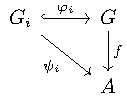
\includegraphics[scale=1.5]{images/fig_1.pdf}\\
                Figura 1. Diagrama conmutativo de $G$ y $A$.
            \end{center}
        \end{minipage}

        esto es, $f\circ\varphi_i=\psi_i$ para todo $i\in I$.
    \end{theor}

    \begin{proof}
        Sean $A$ un grupo abeliano y $\left\{\psi_i\right\}_{ i\in I}$ una familia de homomorfismos tales que
        \begin{equation*}
            \cf{\psi_i}{G_i}{A},\quad\forall i\in I
        \end{equation*}
        sea ahora $x\in G$, como $x_i=e_i,\afa i\in I$ se tiene pues al ser $\psi_i$ homomorfismos debe suceder que $\psi_i(x_i)=e_A,\afa i\in I$ (siendo $e_A$ la identidad de $A$). Por lo cual la suma
        \begin{equation*}
            \sum_{ i\in I}\psi_i(x_i)
        \end{equation*}
        está bien definido (pues solo una cantidad finita de estos elementos es diferente de la identidad). Hacemos
        \begin{equation*}
            f(x)=\sum_{ i\in I}\psi_i(x_i),\quad\forall x\in G
        \end{equation*}
        Veamos que esta función está bien definida, ya se tiene por lo anterior que $\cf{f}{G}{A}$. Sea $x\in G$, si $x$ se expresa como
        \begin{equation*}
            x=\sum_{ j=1}^n y_j \quad\textup{y}\quad x=\sum_{ k=1}^m z_k
        \end{equation*}
        con $y_j,z_k\in G$ para todo $j\in\natint{1,n}$ y para todo $k\in\natint{1,m}$, sea
        \begin{equation*}
            I_0=\left\{i_1,...,i_r \right\}
        \end{equation*}
        el subconjunto de $I$ tal que si $i\in I_0$, entonces
        \begin{equation*}
            {y_j}_i\neq e_i\quad\textup{o}\quad{ z_k}_i\neq e_i 
        \end{equation*}
        para algún $j\in\natint{1,n}$ o algún $k\in\natint{1,m}$. Veamos que
        \begin{equation*}
            \begin{split}
                f\left(\sum_{ j=1}^n y_j \right)&=\sum_{ i\in I}\psi_i\left(\left(\sum_{ j=1}^n y_j\right)_i\right)\\
                &=\sum_{ i\in I_0}\psi_i\left(\sum_{ j=1}^n {y_j}_i\right)\\
                &=\sum_{ i\in I_0}\sum_{ j=1}^n \psi_{ i}\left( {y_j}_{i}\right)\\
            \end{split}
        \end{equation*}
        y,
        \begin{equation*}
            \begin{split}
                f\left(\sum_{ k=1}^m z_k \right)&=\sum_{ i\in I}\psi_i\left(\left(\sum_{ k=1}^m z_k\right)_i\right)\\
                &=\sum_{ i\in I_0}\psi_i\left(\sum_{ k=1}^m {z_k}_i\right)\\
                &=\sum_{ i\in I_0}\sum_{ k=1}^m \psi_{ i}\left( {z_k}_{i}\right)\\
            \end{split}
        \end{equation*}
        por ende,
        \begin{equation*}
            \begin{split}
                f\left(\sum_{ j=1}^n y_j \right)-f\left(\sum_{ k=1}^m z_k \right)&=\sum_{ i\in I_0}\sum_{ j=1}^n \psi_{ i}\left( {y_j}_{i}\right)-\sum_{ i\in I_0}\sum_{ k=1}^m \psi_{ i}\left( {z_k}_{i}\right)\\
                &=\sum_{ i\in I_0}\left(\sum_{ j=1}^n \psi_{ i}\left( {y_j}_{i}\right)-\sum_{ k=1}^m \psi_{ i}\left( {z_k}_{i}\right)\right)\\
                &=\sum_{ i\in I_0}\left(\psi_{ i}\left(\sum_{ j=1}^n {y_j}_{i}\right)-\psi_{ i}\left(\sum_{ k=1}^m{z_k}_{i}\right)\right)\\
                &=\sum_{ i\in I_0}\left(\psi_{ i}\left(\sum_{ j=1}^n {y_j}_{i}\right)-\psi_{ i}\left(\sum_{ k=1}^m{z_k}_{i}\right)\right)\\
                &=\sum_{ i\in I_0}\left(\psi_{ i}\left(\sum_{ j=1}^n {y_j}_{i}-\sum_{ k=1}^m{z_k}_{i}\right)\right)\\
            \end{split}
        \end{equation*}
        %TODO Algo falta aquí sobre la conmutatividad de los $G_i$
        pero $x_i=\sum_ { j=1}^n {y_j}_i$ y $x_i=\sum_ { k=1}^m {z_k}_i$, por lo cual
        \begin{equation*}
            \begin{split}
                f\left(\sum_{ j=1}^n y_j \right)-f\left(\sum_{ k=1}^m z_k \right)&=0\\
                \Rightarrow f\left(\sum_{ j=1}^n y_j \right)&=f\left(\sum_{ k=1}^m z_k \right)\\
            \end{split}
        \end{equation*}
        Se sigue que $f$ está bien definida. Veamos que es homomorfismo. Sean $x,y\in G$, entonces
        \begin{equation*}
            \begin{split}
                f(x+y)&=\sum_{ i\in I}\psi_i(x_i+y_i)\\
                &=\sum_{ i\in I}\psi_i(x_i)+\psi_i(y_i)\\
            \end{split}
        \end{equation*}
        como $A$ es abeliano, esta suma se puede reordenar de cualquier forma, en particular:
        \begin{equation*}
            \begin{split}
                f(x+y)&=\sum_{ i\in I}\psi_i(x_i)+\psi_i(y_i)\\
                &=\sum_{ i\in I}\psi_i(x_i)+\sum_{ i\in I}\psi_i(y_i)\\
                &=f(x)+f(y)\\
            \end{split}
        \end{equation*}
        por lo que $f$ es homomorfismo. Sea ahora $i\in I$, entonces
        \begin{equation*}
            \begin{split}
                f\circ\varphi_i(x_i)&=f(\varphi_i(x_i))\\
                &=\sum_{ j\in I}\psi_j({\varphi_i(x_i)}_j)\\
                &=\psi_i({\varphi_i(x_i)}_i)\\
                &=\psi_i(x_i),\quad\forall x_i\in G_i\\
            \end{split}
        \end{equation*}
        Luego, $f\circ\varphi_i=\psi_i$ para todo $i\in I$. Veamos la unicidad. Para ello, recordemos antes que si $x\in G$, entonces
        \begin{equation*}
            x=\sum_{ i\in I}\varphi_i(x_i)
        \end{equation*}
        (básicamente $x$ se expresa como la suma de sus componentes una por una vistas como elementos de $G$) siendo esta suma finita y por ende, está bien definida. Si $\cf{g}{G}{A}$ es otro homomorfismo tal que
        \begin{equation*}
            g\circ\varphi_i=\psi_i,\quad\forall i\in I
        \end{equation*}
        se tiene que
        \begin{equation*}
            \begin{split}
                g(x)&=g\left(\sum_{ i\in I}\varphi_i(x_i)\right)\\
                &=\sum_{ i\in I} g\circ\varphi_i(x_i)\\
                &=\sum_{ i\in I}\psi_i(x_i)\\
                &=f(x),\quad\forall x\in G\\
            \end{split}
        \end{equation*}
        por ende, $f$ es único.
    \end{proof}

    Este teorema caracteriza la suma directa de grupos abelianos, como lo muestra la siguiente proposición.

    \begin{propo}
        \label{caractSumDir_2}
        Sea $\left\{G_i \right\}_{ i\in I}$ una familia de grupos abelianos y $G=\bigoplus_{ i\in I}G_i$; sea $G'$ un subgrupo abeliano y consideremos para cada $i\in I$ las funciones $\cf{\varphi_i'}{G_i}{G'}$ tales que la conclusión del Teorema \ref{caractSumDir_1} cambiando a $G'$ por 
    \end{propo}

    \begin{proof}
        
    \end{proof}



    \section{Grupos Abelianos Libres}

    Recordemos que si $G$ es un grupo, decimos que un conjunto $S\subseteq G$ \textbf{genera a $G$}, si
    \begin{equation*}
        G=\left\{s_1^{\epsilon_1}\cdot\dots\cdot s_m^{\epsilon_m}\Big|s_i\in S,\forall i\in\natint{1,m}; m\in\mathbb{N} \right\}
    \end{equation*}
    y en tal caso, se denota $G=\langle S\rangle$. 

    \begin{exa}
        Si $G$ es un grupo cíclico de orden $n\in\mathbb{N}$, entonces existe $x\in G$ tal que $G=\langle x\rangle$, así que
        \begin{equation*}
            G=\left\{x,x^2,...,x^n=e\right\}
        \end{equation*}
    \end{exa}

    \begin{mydef}
        Sea $S$ un conjunto arbitrario. Un \textbf{grupo abeliano libre} en el conjunto $S$ es un grupo abeliano $F$ junto con una función $\cf{f}{S}{F}$ tal que se cumple la siguiente condición:
        \begin{itemize}
            \item Para cualquier grupo abeliano y cualquier función $\cf{\psi}{S}{A}$, existe un único homomorfismo $\cf{f}{F}{A}$ tal que el diagrama:
            
            \begin{minipage}{\textwidth}
                \begin{center}
                    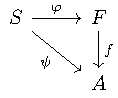
\includegraphics[scale=1.5]{images/fig_2.pdf}\\
                    Figura 2. Diagrama conmutativo de $F$ y $A$.
                \end{center}
            \end{minipage}
            
            es conmutativo.
        \end{itemize}
    \end{mydef}

    %TODO

\end{document}